\documentclass[a4paper,12pt]{report}
\usepackage[utf8]{inputenc}
\usepackage{fontenc}
\usepackage[french, arabic]{babel} % If you write in French
\usepackage{a4wide}
\usepackage{graphicx}
\usepackage{placeins}
%pour la mise en page des tableaux
\usepackage{array}
\usepackage{tabularx}
\usepackage[table,xcdraw]{xcolor}
\usepackage{wrapfig}
\usepackage{subcaption}
\usepackage{color, colortbl}
\definecolor{Gray}{gray}{0.9}
\definecolor{LightCyan}{rgb}{0.88,1,1}
\usepackage{longtable}
\usepackage{float}
\usepackage{array} % for extrarowheight
\usepackage{lscape}
\usepackage{afterpage}
\usepackage{rotating}
\usepackage[nottoc,notlof,notlot]{tocbibind}
\usepackage{tocloft}
\usepackage{pdfpages}
\graphicspath{{images/}{images_pfe/}}
\newlength\figureheight
\newlength\figurewidth
\usepackage{ifthen}
\usepackage{ifpdf}
\ifpdf
\usepackage[pdftex]{hyperref}
\else
\usepackage{hyperref}
\fi
\usepackage{color}
\hypersetup{%
colorlinks=true,
linkcolor=black,
citecolor=black,
urlcolor=blue}
% \urlstyle{same}
\usepackage[top=2.5cm,bottom=2.5cm,right=2.5cm,left=2.5cm]{geometry}
\usepackage{changepage}

\usepackage{tabularx}
    \newcolumntype{L}{>{\raggedright\arraybackslash}X}
\usepackage{longtable}

\usepackage{xltabular}
\renewcommand{\tablename}{Tableau}
\renewcommand{\figurename}{Figure}



%pour les références bibliographiques
\usepackage[citestyle=authoryear,bibstyle=authoryear,doi=false,isbn=false,eprint=false,maxcitenames=1,uniquelist=false,backend=biber]{biblatex}
\addbibresource{references.bib}

\AtEveryBibitem{
  \ifentrytype{misc}{
  }{
    \clearfield{url}
    \clearfield{urlyear}
    
  }
}
%% pour la numération des sous sou sections
\setcounter{tocdepth}{2}
\setcounter{secnumdepth}{2}



% pour les algorithmes
\usepackage[ruled,vlined,linesnumbered]{algorithm2e}
\DontPrintSemicolon

\setlength\arrayrulewidth{1pt}
\renewcommand{\baselinestretch}{1.05}
\usepackage{fancyhdr}
\pagestyle{fancy}
\fancyhf{}
\lhead{\bfseries\nouppercase{\leftmark}}
\rfoot{\bfseries\thepage}
\setlength{\headheight}{14.5pt}

\let\headruleORIG\headrule

\renewcommand{\headrule}{\color{black} \headruleORIG}
\renewcommand{\headrulewidth}{1.0pt}
\usepackage{colortbl}
\arrayrulecolor{black}

\fancypagestyle{plain}{
  \fancyhead{}
  \fancyfoot[R]{\bfseries\thepage}
  \renewcommand{\headrulewidth}{0pt}
}



\makeatletter
\def\@textbottom{\vskip \z@ \@plus 1pt}
\let\@texttop\relax
\makeatother

\makeatletter
\def\cleardoublepage{\clearpage\if@twoside \ifodd\c@page\else%
  \hbox{}%
  \thispagestyle{empty}%
  \newpage%
  \if@twocolumn\hbox{}\newpage\fi\fi\fi}
\makeatother

\usepackage{amsthm}
\usepackage{amssymb,amsmath,bbm}
\usepackage{array}
\usepackage{bm}
\usepackage{multirow}
\usepackage[footnote]{acronym}

\usepackage[bottom]{footmisc}






\newtheoremstyle{break}
  {11pt}{11pt}%
  {\itshape}{}%
  {\bfseries}{}%
  {\newline}{}%
\theoremstyle{break}

%\theoremstyle{definition}
\newtheorem{definition}{Définition}[chapter]

%\theoremstyle{definition}
\newtheorem{theoreme}{Théorème}[chapter]

%\theoremstyle{remark}
\newtheorem{remarque}{Remarque}[chapter]

%\theoremstyle{plain}
\newtheorem{propriete}{Propriété}[chapter]
\newtheorem{exemple}{Exemple}[chapter]

%table break line

\usepackage{makecell}

\renewcommand\theadalign{bl}
\renewcommand\theadfont{\bfseries}
\renewcommand\cellalign{bl}
\renewcommand\cellgape{\Gape[2pt]}

\parskip=5pt
%\sloppy
 %%%%********************************************************************
\usepackage{xcolor}
\definecolor{quotemark}{gray}{0.7}
\makeatletter
\def\fquote{%
    \@ifnextchar[{\fquote@i}{\fquote@i[]}%]
           }%
\def\fquote@i[#1]{%
    \def\tempa{#1}%
    \@ifnextchar[{\fquote@ii}{\fquote@ii[]}%]
                 }%
\def\fquote@ii[#1]{%
    \def\tempb{#1}%
    \@ifnextchar[{\fquote@iii}{\fquote@iii[]}%]
                      }%
\def\fquote@iii[#1]{%
    \def\tempc{#1}%
    \vspace{1em}%
    \noindent%
    \begin{list}{}{%
         \setlength{\leftmargin}{0.1\textwidth}%
         \setlength{\rightmargin}{0.1\textwidth}%
                  }%
         \item[]%
         \begin{picture}(0,0)%
         \put(-15,-5){\makebox(0,0){\scalebox{3}{\textcolor{quotemark}{``}}}}%
         \end{picture}%
         \begingroup\itshape}%
 %%%%********************************************************************
 \def\endfquote{%
 \endgroup\par%
 \makebox[0pt][l]{%
 \hspace{0.8\textwidth}%
 \begin{picture}(0,0)(0,0)%
 \put(15,15){\makebox(0,0){%
 \scalebox{3}{\color{quotemark}''}}}%
 \end{picture}}%
 \ifx\tempa\empty%
 \else%
    \ifx\tempc\empty%
       \hfill\rule{100pt}{0.5pt}\\\mbox{}\hfill\tempa,\ \emph{\tempb}%
   \else%
       \hfill\rule{100pt}{0.5pt}\\\mbox{}\hfill\tempa,\ \emph{\tempb},\ \tempc%
   \fi\fi\par%
   \vspace{0.5em}%
 \end{list}%
 }%
 \makeatother
 %%%%********************************************************************
 
 
 \usepackage{afterpage}

\newcommand\blankpage{%
    \null
    \thispagestyle{empty}%
    \addtocounter{page}{-1}%
    \newpage}
    
\renewcommand{\listalgorithmcfname}{Liste des algorithmes}
\usepackage{polyglossia}
\setmainlanguage{french}
\setotherlanguage{arabic}
\newfontfamily\arabicfont[Script=Arabic,Scale=1.3]{Scheherazade}

\newcommand{\mychapter}[2]{
    
    \chapter*{#2}
    \addcontentsline{toc}{chapter}{#2}
}

\usepackage[page,toc,titletoc,title]{appendix}

\addto\captionsfrench{%
  \renewcommand\appendixname{Annexe}
  \renewcommand\appendixpagename{Annexes}
  \renewcommand{\appendixtocname}{Annexes}
}
\usepackage{etoolbox}
\appto\appendix{\addtocontents{toc}{\protect\setcounter{tocdepth}{0}}}

% reinstate the correct level for list of tables and figures and algorithms
\appto\listoffigures{\addtocontents{lof}{\protect\setcounter{tocdepth}{1}}}
\appto\listoftables{\addtocontents{lot}{\protect\setcounter{tocdepth}{1}}}
\appto\listofalgorithms{\addtocontents{loa}{\protect\setcounter{tocdepth}{1}}}



\begin{document}


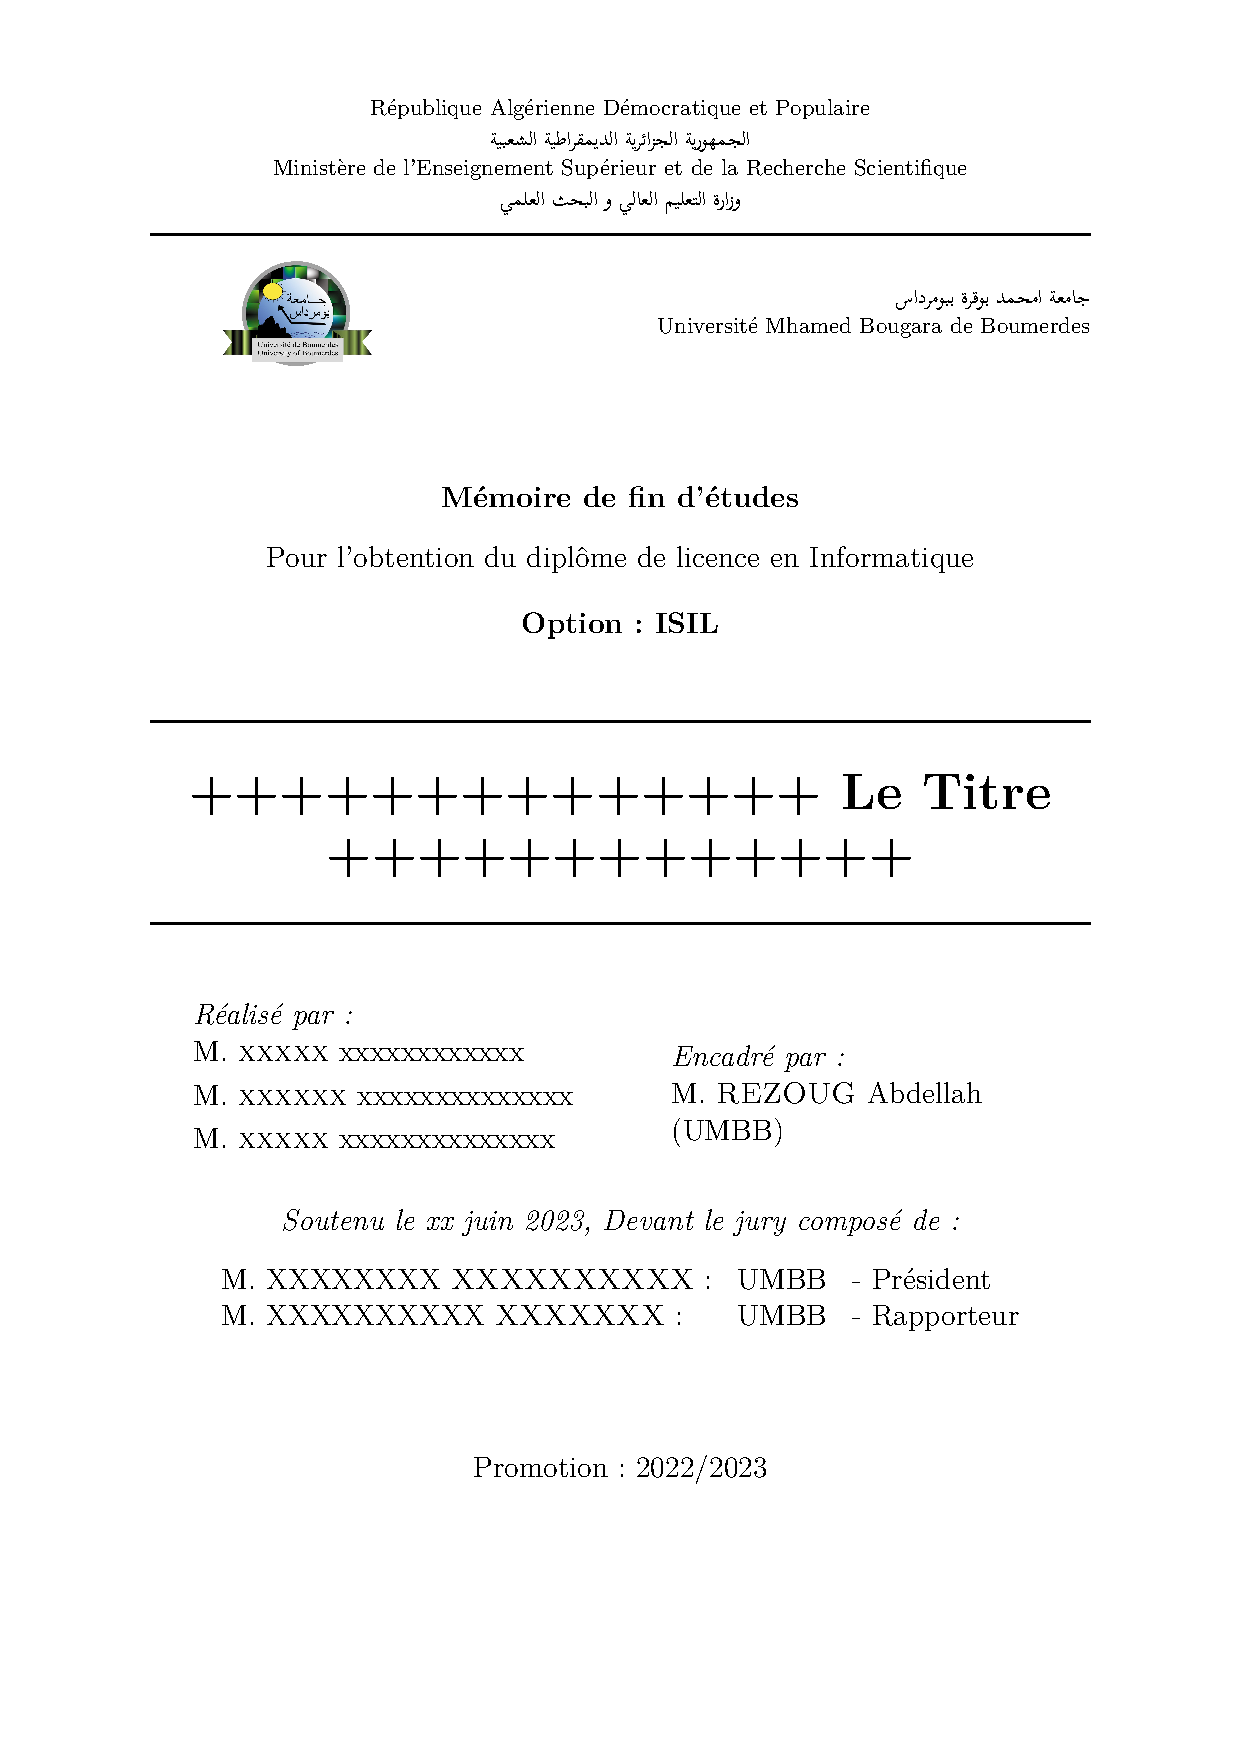
\includepdf[pages=-]{00-Page-de-garde.pdf}
\pagenumbering{Roman}
%\thispagestyle{empty}
\vspace*{2cm}
\begin{center}
    \huge{\textbf{\textit{Note de confidentialité}}}
\end{center}
\bigskip
\medskip 
\vspace{2cm}
\begin{center}
\large{
ertaines informations présentes dans ce mémoire ont été floutées par soucis de confidentialité. Merci pour votre compréhension.
}
\end{center}



\clearpage

\mychapter{0}{Dédicace}

\begin{fquote}
\begin{center}
\large{

\uppercase{à} mLorem ipsum dolor sit amet, consectetur adipiscing elit. Proin posuere euismod neque, non semper nibh viverra sed. Praesent ut varius magna. Fusce ipsum ante, semper nec interdum at, semper et lacus. Nulla ultrices magna a fringilla finibus,\\[12pt]
\uppercase{à} Lorem ipsum dolor sit amet, consectetur adipiscing elit. Proin posuere euismod neque, non semper nibh viverra sed. Praesent ut varius magna. Fusce ipsum ante, semper nec interdum at, semper et lacus. Nulla ultrices magna a fringilla finibus,\\[12pt]
\uppercase{à} Lorem ipsum dolor sit amet, consectetur adipiscing elit. Proin posuere euismod neque, non semper nibh viverra sed. Praesent ut varius magna. Fusce ipsum ante, semper nec interdum at, semper et lacus. Nulla ultrices magna a fringilla finibus,\\[12pt]
\uppercase{à} tous ceux qui me sont chers, à vous tous\\[12pt]
Merci.
}
\end{center}
\bigskip
\medskip
\end{fquote}

\begin{adjustwidth}{2cm}{1cm}
\hspace*{\fill} \textbf{\textit{\large{- nOM}}}
\end{adjustwidth}

\clearpage
\mychapter{0}{Remerciements}

Tout d'abord, je remercie Allah le tout puissant de m'avoir donné le courage et la patience nécessaires à mener ce travail à son terme.

Je tiens à remercier tout particulièrement mon encadrant \textbf{nom encadreur}, pour l’aide compétente qu’il m’a apportée, pour sa patience et son encouragement. Son œil critique m’a été très précieux pour structurer le travail et pour améliorer la qualité des différentes sections.

Je tiens à remercier également mon promoteur \textbf{Nom promoteur} pour son aide immense, la qualité de son suivie ainsi que pour tous les conseils et les informations qu'il m’a prodigués avec un degré de patience et de professionnalisme sans égal.

Je tiens aussi à adresser mes plus sincères remerciements à \textbf{xxxxxxxxxxx}, manager du service Big Data \& Data Analytics Platforms pour m'offrir l'opportunité d'intégrer son équipe et pour son soutien.

Un très grand remerciement et une très grande reconnaissance sont destinés à \textbf{xxxxxxxxxxx} de m'avoir aidé à obtenir ce stage de fin d'études chez xxxxx.



Pour finir, je souhaite remercier toute personne ayant contribué de prés ou de loin à la réalisation de ce travail.

\clearpage
\mychapter{0}{Résumé}

ici résumé...
\medskip

ici résumé...

\vspace{1cm}


\noindent\rule[2pt]{\textwidth}{0.5pt}

{\textbf{Mots clés :}}
Ici mot clé
\\
\noindent\rule[2pt]{\textwidth}{0.5pt}

\clearpage

\mychapter{0}{Abstract}

Here abstract...

\medskip

Here abstract...

\vspace{1cm}



\noindent\rule[2pt]{\textwidth}{0.5pt}

{\textbf{Keywords :}}
here keywords
\\
\noindent\rule[2pt]{\textwidth}{0.5pt}


\chapter*{\hfill \begin{Arabic} ملخص \end{Arabic}}

\begin{Arabic}
\addcontentsline{toc}{chapter}{ ملخص}
\end{Arabic}


 

\begin{Arabic}
قد كان المجتمع المدني منذ القرن التاسع عشر موضوع إحالة في الخطاب الفلسفي وكذلك في الخطاب السياسي بوصفه هذه الواقعة التي تفرض نفسها، والتي تقاوم وتُخضع وتتفلت من الحكومة أو من الدولة أو من جهاز الدولة أو من المؤسسة. .

\end{Arabic}

\medskip

\begin{Arabic}أعتقد أنه يجب أن نكون حذرين للغاية بالنسبة إلى الحقيقة والواقع الذي ننسبه إلى هذا المجتمع المدني، إنه ليس هذا المُعطى التاريخي-الطبيعي الذي يأتي وكأنه يقوم بدور القاعدة/الأرضية، أو أنه أيضًا مبدأ لمعارضة الدولة والمؤسسات السياسية، ليس المجتمع المدني واقعة أولية ومباشرة، إن المجتمع المدني هو جزء من تكنولوجيا الحكمانية الحديثة، والقول إنه يمثل جزءًا لا يعني أنه منتج لا أكثر ولا أقل، ولا يعني أيضًا أنه ليس واقعًا أو حقيقة، إن المجتمع المدني، مثله مثل الجنون أو الجنسانية، إنه مثل تلك الوقائع التي أسميها وقائع التسويات والصفقات، بمعنى أنه يدخل ضمن اللعبة الخاصة بعلاقات السلطة، ولما ينفلت منها، بحيث يولد وينشأ شيء ما على الحد الفاصل بين الحكّام والمحكومين، وفي هذه الوجوه والصور التبادلية والمؤقتة إلّا أنها مع ذلك ليست أقل واقعية وحقيقة، وهذا هو الذي نسميه المجتمع المدني أو الجنون أو الجنسانية .. إلخ. .
\end{Arabic}

\medskip

\begin{Arabic}
إذن: المجتمع المدني بوصفه عنصرًا ناتجًا من واقع التسوية في تاريخ تكنولوجيات الحكمانية، علاقة تسوية تبدو لي متلازمة تمامًا مع هذا الشكل من تكنولوجيا الحكمانية التي نسميها ليبرالية، بمعنى: تكنولوجيا حكم لها هدف هو حدّها الذاتي المرتبط بخصوص العمليات الاقتصادية
\end{Arabic}

\medskip

\vspace{3cm}

\noindent\rule[2pt]{\textwidth}{0.5pt}


\begin{Arabic}
\textbf{كلمات مفتاحية :}

تحسين المسارات ، مشكلة البائع المتجول مع قيود دورية ، تعلم الآلة ، التصنيف.

\end{Arabic}

\noindent\rule[2pt]{\textwidth}{0.5pt}



\renewcommand{\cftpartleader}{\cftdotfill{\cftdotsep}} 
\renewcommand{\cftchapleader}{\cftdotfill{\cftdotsep}} 
\tableofcontents
\clearpage
\listoffigures
\clearpage
\listoftables
\clearpage
\listofalgorithms

\clearpage
\chapter*{Liste des sigles et acronymes}
\begin{acronym}[CP-OFDMX] % Give the longest acronym here

\acro{ACP}{\emph{Analyse en Composantes Principales}}
\medskip

\acro{API}{\emph{Application Programming Interface}}
\medskip

\acro{ARPT}{\emph{Autorité de Régulation de la Poste et des Télécommunications}}
\medskip

\acro{BTS}{\emph{Base Transceiver Station}}
\medskip

\acro{DBSS}{\emph{Digital Business Support System}}
\medskip

\acro{DWH}{\emph{Data Warehouse}}
\medskip

\acro{ETL}{\emph{Extraction Transformtion Load}}
\medskip

\acro{HTTP}{\emph{Hypertext Transfer Protocol }}
\medskip

\acro{JSON}{\emph{JavaScript Object Notation}}
\medskip

\acro{KDE}{\emph{Kernel Density Estimation}}
\medskip

\acro{OTA}{\emph{Optimum Telecom Algeria}}
\medskip

\acro{PTSP}{\emph{Periodic Traveling Salesman Problem}}
\medskip

\acro{PVRP}{\emph{Periodic Vehicle Routing Problem}}
\medskip

\acro{REST}{\emph{Representational State Transfer}}
\medskip

\acro{SIM}{\emph{Subscriber Identification Module}}
\medskip



\acro{SVM}{\emph{Support Vector Machine}}
\medskip


\acro{TSP}{\emph{Traveling Salesman Problem}}
\medskip

\acro{VRP}{\emph{Vehicle Routing Problem}}
\medskip


\end{acronym}

%%%%%%%%%%%%%%%%%%%%%%%%%%%%%%%%%%%%%%%%%%%%
%%% Content of the report and references %%%
%%%%%%%%%%%%%%%%%%%%%%%%%%%%%%%%%%%%%%%%%%%%

\cleardoublepage

\pagenumbering{arabic}
\chapter*{Introduction générale}
\addcontentsline{toc}{chapter}{Introduction générale}
\markboth{Introduction générale}{Introduction générale}
\label{chap:introduction}
%\minitoc

\section*{Contexte}

\medskip

\section*{Problématique}



\section*{Objectifs}





\section*{Organisation du mémoire}

Ce mémoire est organisé en six chapitres :

\medskip





\chapter{État de l'art}

\clearpage


\section{Introduction}

\chapter{Étude de l'existant}
\clearpage
\label{sec:organisme}

\section{Introduction}


\medskip

\section{Conclusion}

%%% mode: latex
%%% TeX-master: "isae-report-template"
%%% End: 
\chapter{Expression des besoins}
\clearpage
\label{chap:besoins}

\section{Introduction}


\section{Conclusion}





%%% Local Variabs prles: 
%%% mode: latex
%%% TeX-master: "isae-report-template"
%%% End: 
\chapter{Conception}

\newpage

\section{Introduction}

\begin{figure}[hbt!]
  \centering
  
\includegraphics[height=10cm]{images_pfe/Logo_umbb.png}
  \caption{Partie serveur.}
  \label{fig:server-side}
\end{figure}
\FloatBarrier

\medskip




\begin{figure}[hbt!]
  \centering
  
\includegraphics[height=10cm]{images_pfe/Logo_umbb.png}
  \caption{Partie client.}
  \label{fig:client-side}
\end{figure}
\FloatBarrier



\section{Conclusion}



\chapter{Réalisation}

\newpage

\section{Introduction}

\section{Conclusion}





\chapter*{Conclusion et perspectives}
\addcontentsline{toc}{chapter}{Conclusion et perspectives}
\markboth{Conclusion et perspectives}{Conclusion et perspectives}
\label{sec:conclusion}

\clearpage

\section*{Conclusion générale}

  ici conclusion....
    
   
    
    
    

\section*{Perspectives}

   ici perspectives
    
    
\section*{Appréciation personnelle}

    ici appréciation...





    

%%% Local Variables: 
%%% mode: latex
%%% TeX-master: "isae-report-template"
%%% End: 



%choix du style de la biblio

\printbibliography[nottype=misc,title={Bibliographie}]
 
\printbibliography[type=misc,title={Webographie}]





\appendix
\appendixpage

\chapter{Définitions}
\label{app:definitions}
\chapter{Partie données}







\clearpage
\thispagestyle{empty}




\end{document}
